% 2-15-rb-tree.tex

%%%%%%%%%%%%%%%%%%%%
\documentclass[a4paper, justified]{tufte-handout}

% hw-preamble.tex

% geometry for A4 paper
% See https://tex.stackexchange.com/a/119912/23098
\geometry{
  left=20.0mm,
  top=20.0mm,
  bottom=20.0mm,
  textwidth=130mm, % main text block
  marginparsep=5.0mm, % gutter between main text block and margin notes
  marginparwidth=50.0mm % width of margin notes
}

% for colors
\usepackage{xcolor} % usage: \color{red}{text}
% predefined colors
\newcommand{\red}[1]{\textcolor{red}{#1}} % usage: \red{text}
\newcommand{\blue}[1]{\textcolor{blue}{#1}}
\newcommand{\teal}[1]{\textcolor{teal}{#1}}

\usepackage{todonotes}

% heading
\usepackage{sectsty}
\setcounter{secnumdepth}{2}
\allsectionsfont{\centering\huge\rmfamily}

% for Chinese
\usepackage{xeCJK}
\usepackage{zhnumber}
\setCJKmainfont[BoldFont=FandolSong-Bold.otf]{FandolSong-Regular.otf}

% for fonts
\usepackage{fontspec}
\newcommand{\song}{\CJKfamily{song}} 
\newcommand{\kai}{\CJKfamily{kai}} 

% To fix the ``MakeTextLowerCase'' bug:
% See https://github.com/Tufte-LaTeX/tufte-latex/issues/64#issuecomment-78572017
% Set up the spacing using fontspec features
\renewcommand\allcapsspacing[1]{{\addfontfeature{LetterSpace=15}#1}}
\renewcommand\smallcapsspacing[1]{{\addfontfeature{LetterSpace=10}#1}}

% for url
\usepackage{hyperref}
\hypersetup{colorlinks = true, 
  linkcolor = teal,
  urlcolor  = teal,
  citecolor = blue,
  anchorcolor = blue}

\newcommand{\me}[4]{
    \author{
      {\bfseries 姓名:}\underline{#1}\hspace{2em}
      {\bfseries 学号:}\underline{#2}\hspace{2em}\\[10pt]
      {\bfseries 评分:}\underline{#3\hspace{3em}}\hspace{2em}
      {\bfseries 评阅:}\underline{#4\hspace{3em}}
  }
}

% Please ALWAYS Keep This.
\newcommand{\noplagiarism}{
  \begin{center}
    \fbox{\begin{tabular}{@{}c@{}}
      请独立完成作业,不得抄袭。\\
      若得到他人帮助, 请致谢。\\
      若参考了其它资料,请给出引用。\\
      鼓励讨论,但需独立书写解题过程。
    \end{tabular}}
  \end{center}
}

\newcommand{\goal}[1]{
  \begin{center}{\fcolorbox{blue}{yellow!60}{\parbox{0.50\textwidth}{\large 
    \begin{itemize}
      \item 体会``思维的乐趣''
      \item 初步了解递归与数学归纳法 
      \item 初步接触算法概念与问题下界概念
    \end{itemize}}}}
  \end{center}
}

% Each hw consists of four parts:
\newcommand{\beginrequired}{\hspace{5em}\section{作业 (必做部分)}}
\newcommand{\beginoptional}{\section{作业 (选做部分)}}
\newcommand{\beginot}{\section{Open Topics}}
\newcommand{\begincorrection}{\section{订正}}
\newcommand{\beginfb}{\section{反馈}}

% for math
\usepackage{amsmath, mathtools, amsfonts, amssymb}
\newcommand{\set}[1]{\{#1\}}

% define theorem-like environments
\usepackage[amsmath, thmmarks]{ntheorem}

\theoremstyle{break}
\theorempreskip{2.0\topsep}
\theorembodyfont{\song}
\theoremseparator{}
\newtheorem{problem}{题目}[subsection]
\renewcommand{\theproblem}{\arabic{problem}}
\newtheorem{ot}{Open Topics}

\theorempreskip{3.0\topsep}
\theoremheaderfont{\kai\bfseries}
\theoremseparator{:}
\theorempostwork{\bigskip\hrule}
\newtheorem*{solution}{解答}
\theorempostwork{\bigskip\hrule}
\newtheorem*{revision}{订正}

\theoremstyle{plain}
\newtheorem*{cause}{错因分析}
\newtheorem*{remark}{注}

\theoremstyle{break}
\theorempostwork{\bigskip\hrule}
\theoremsymbol{\ensuremath{\Box}}
\newtheorem*{proof}{证明}

% \newcommand{\ot}{\blue{\bf [OT]}}

% for figs
\renewcommand\figurename{图}
\renewcommand\tablename{表}

% for fig without caption: #1: width/size; #2: fig file
\newcommand{\fig}[2]{
  \begin{figure}[htbp]
    \centering
    \includegraphics[#1]{#2}
  \end{figure}
}
% for fig with caption: #1: width/size; #2: fig file; #3: caption
\newcommand{\figcap}[3]{
  \begin{figure}[htbp]
    \centering
    \includegraphics[#1]{#2}
    \caption{#3}
  \end{figure}
}
% for fig with both caption and label: #1: width/size; #2: fig file; #3: caption; #4: label
\newcommand{\figcaplbl}[4]{
  \begin{figure}[htbp]
    \centering
    \includegraphics[#1]{#2}
    \caption{#3}
    \label{#4}
  \end{figure}
}
% for margin fig without caption: #1: width/size; #2: fig file
\newcommand{\mfig}[2]{
  \begin{marginfigure}
    \centering
    \includegraphics[#1]{#2}
  \end{marginfigure}
}
% for margin fig with caption: #1: width/size; #2: fig file; #3: caption
\newcommand{\mfigcap}[3]{
  \begin{marginfigure}
    \centering
    \includegraphics[#1]{#2}
    \caption{#3}
  \end{marginfigure}
}

\usepackage{fancyvrb}

% for algorithms
\usepackage[]{algorithm}
\usepackage[]{algpseudocode} % noend
% See [Adjust the indentation whithin the algorithmicx-package when a line is broken](https://tex.stackexchange.com/a/68540/23098)
\newcommand{\algparbox}[1]{\parbox[t]{\dimexpr\linewidth-\algorithmicindent}{#1\strut}}
\newcommand{\hStatex}[0]{\vspace{5pt}}
\makeatletter
\newlength{\trianglerightwidth}
\settowidth{\trianglerightwidth}{$\triangleright$~}
\algnewcommand{\LineComment}[1]{\Statex \hskip\ALG@thistlm \(\triangleright\) #1}
\algnewcommand{\LineCommentCont}[1]{\Statex \hskip\ALG@thistlm%
  \parbox[t]{\dimexpr\linewidth-\ALG@thistlm}{\hangindent=\trianglerightwidth \hangafter=1 \strut$\triangleright$ #1\strut}}
\makeatother

% for footnote/marginnote
% see https://tex.stackexchange.com/a/133265/23098
\usepackage{tikz}
\newcommand{\circled}[1]{%
  \tikz[baseline=(char.base)]
  \node [draw, circle, inner sep = 0.5pt, font = \tiny, minimum size = 8pt] (char) {#1};
}
\renewcommand\thefootnote{\protect\circled{\arabic{footnote}}} % feel free to modify this file
%%%%%%%%%%%%%%%%%%%%
\title{第3-14讲: 平面图与图的染色}
\me{林凡琪}{211240042}{}{}
\date{\zhtoday} % or like 2019年9月13日
%%%%%%%%%%%%%%%%%%%%
\begin{document}
\maketitle
%%%%%%%%%%%%%%%%%%%%
\noplagiarism % always keep this line
%%%%%%%%%%%%%%%%%%%%
\begin{abstract}
  % \begin{center}{\fcolorbox{blue}{yellow!60}{\parbox{0.65\textwidth}{\large 
  %   \begin{itemize}
  %     \item 
  %   \end{itemize}}}}
  % \end{center}
\end{abstract}
%%%%%%%%%%%%%%%%%%%%
\beginrequired

%%%%%%%%%%%%%%%
\begin{problem}[CZ 9.3]
\end{problem}

\begin{solution}
  We can know that:
  \begin{equation}
    p=
    \left\{
    \begin{array}{ll}
      1,                          & f(x_1)\leq f(x) \\
      e^{-\frac{f(x_1)-f(x)}{T}}, & f(x_1)> f(x)
    \end{array}
    \right.
  \end{equation}
  \\
  (a)
  $m = \frac{(3+4+4+4+5+6+6)}{2} = 16, n = 6$.\\
  For $m> 3n - 6$, so G is nonplanar.\\
  \\
  (b)
  $m = \frac{(4+4+4+5+5+5+6+6+6+7+7+7)}{2} = 33, n = 12$.\\
  For $m> 3n - 6$, so G is nonplanar.
\end{solution}
%%%%%%%%%%%%%%%

%%%%%%%%%%%%%%%
\begin{problem}[CZ 9.5]
\end{problem}

\begin{solution}
  (a)
  \begin{figure}[htbp]
    \centering
    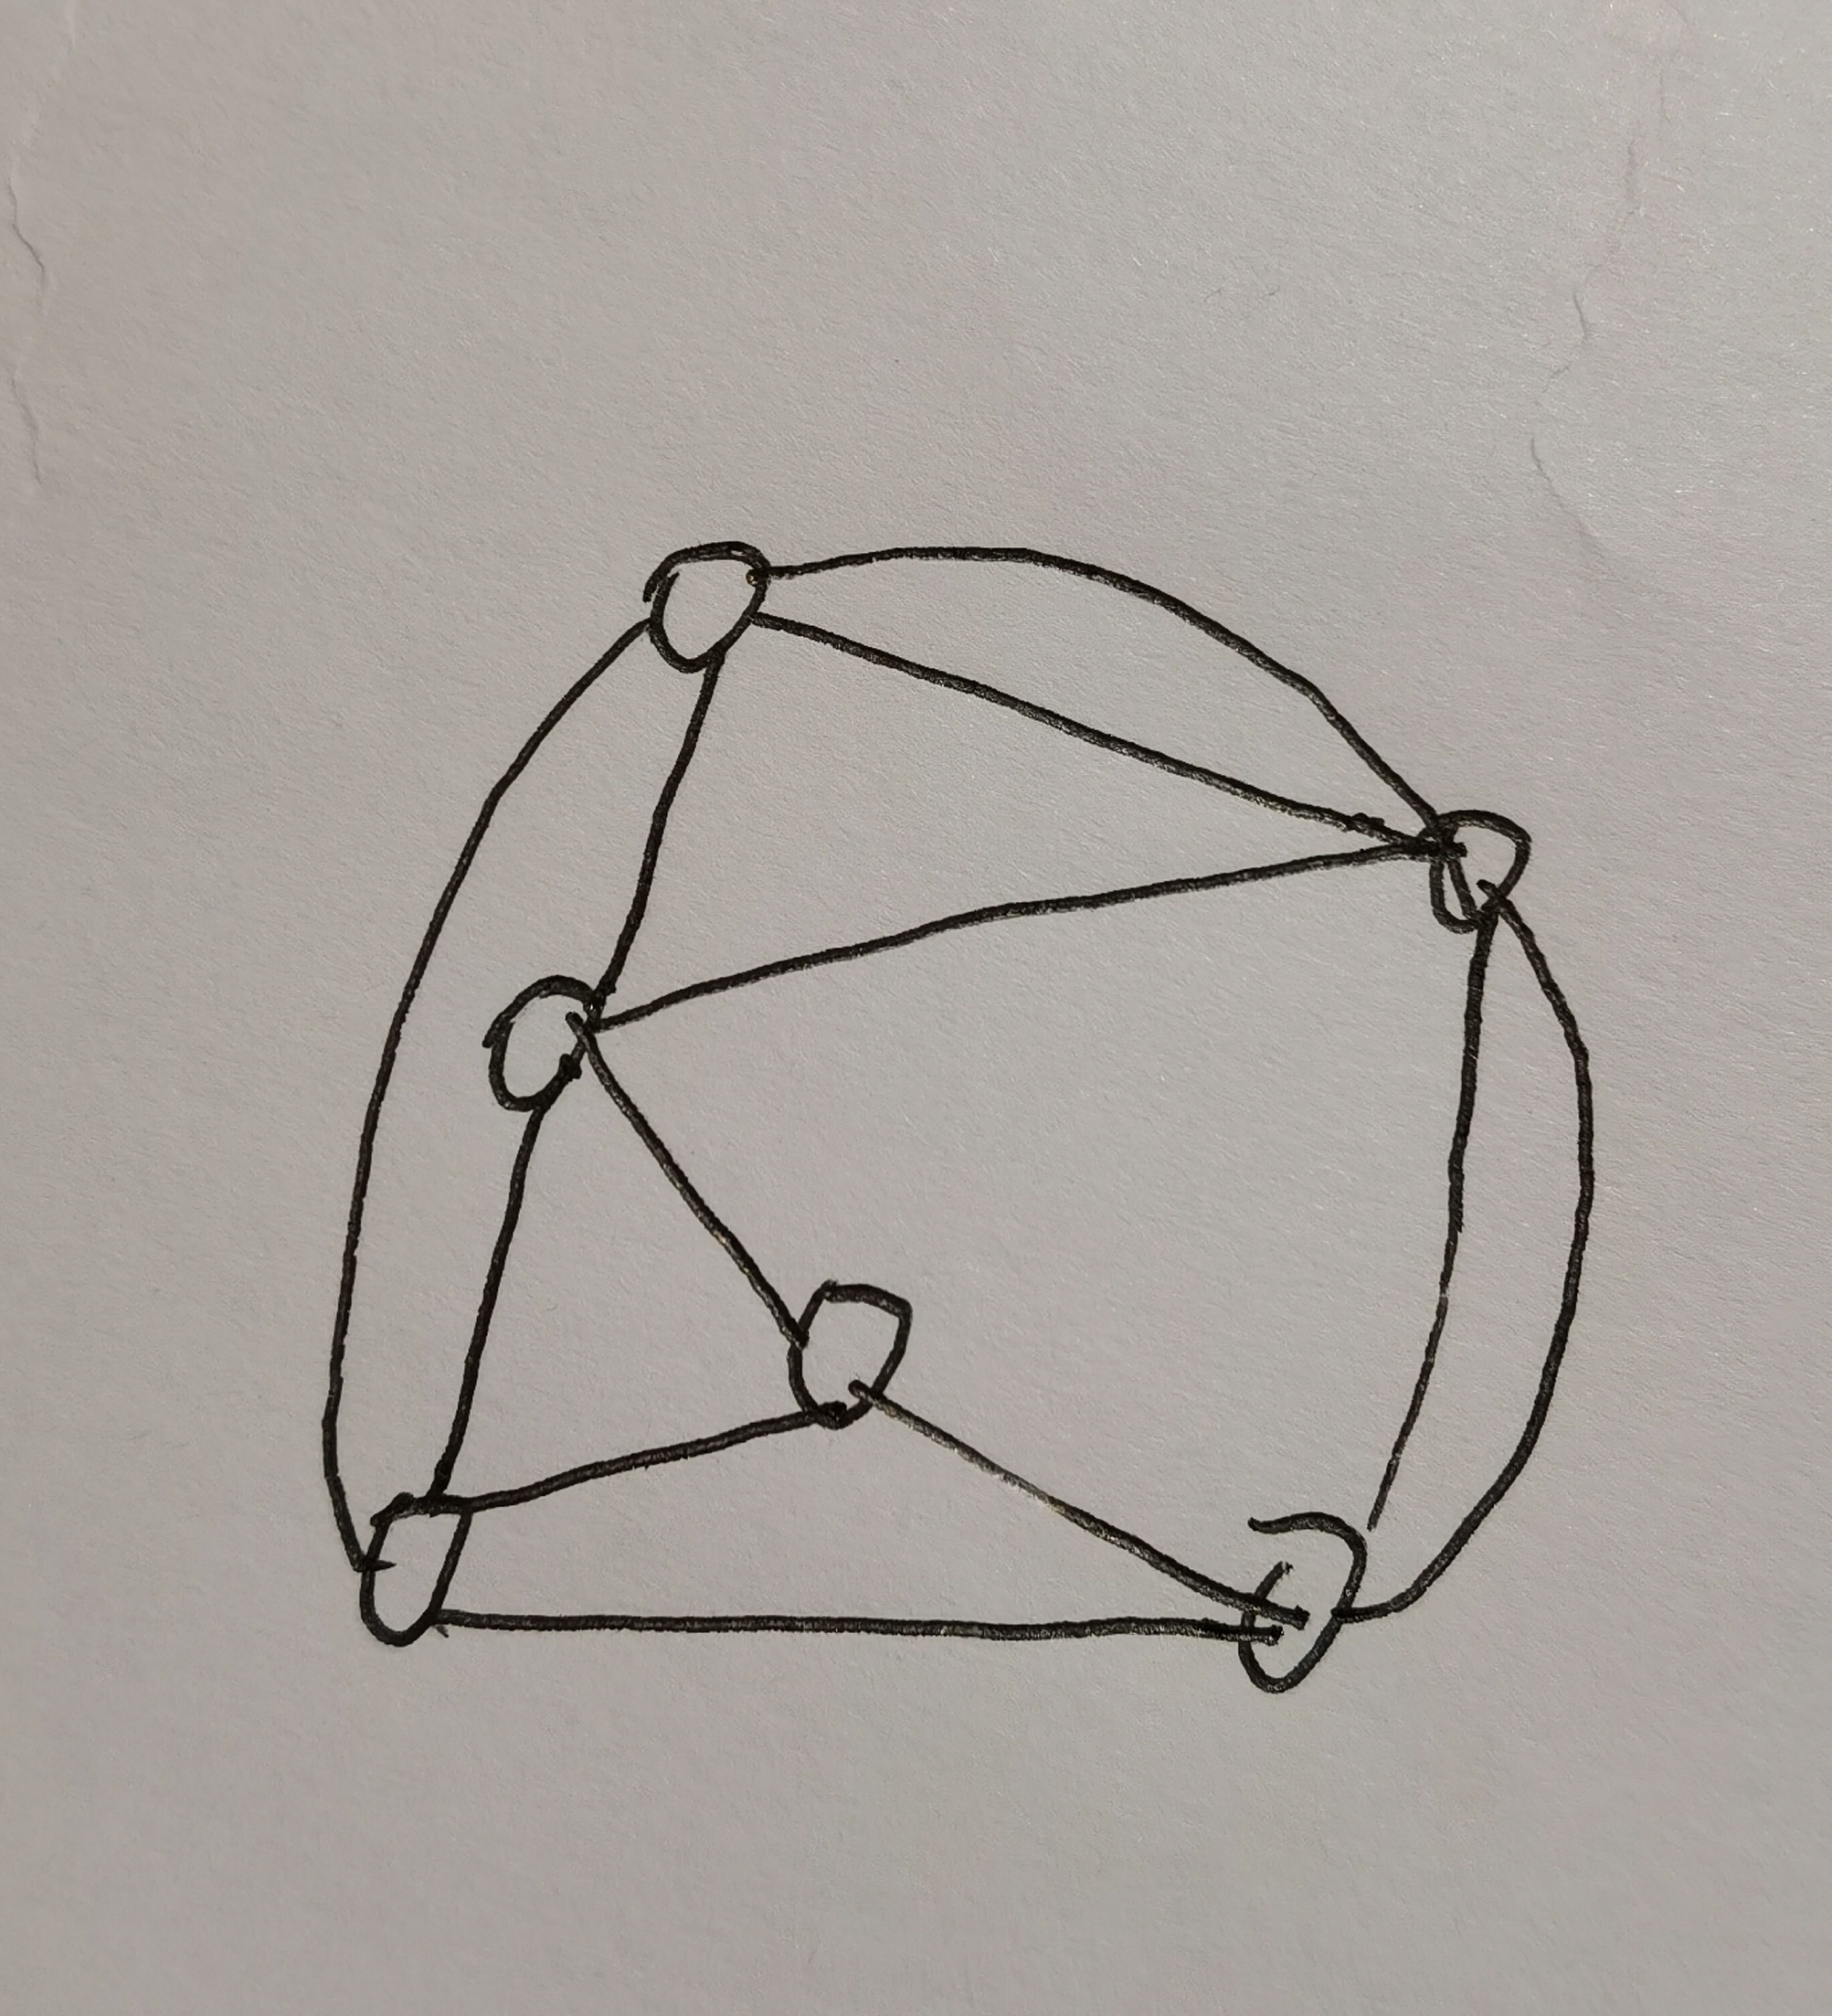
\includegraphics[width = 0.30\linewidth]{figs/a}
  \end{figure}
  \\
  $K_5$\\
  (b)
  \begin{figure}[htbp]
    \centering
    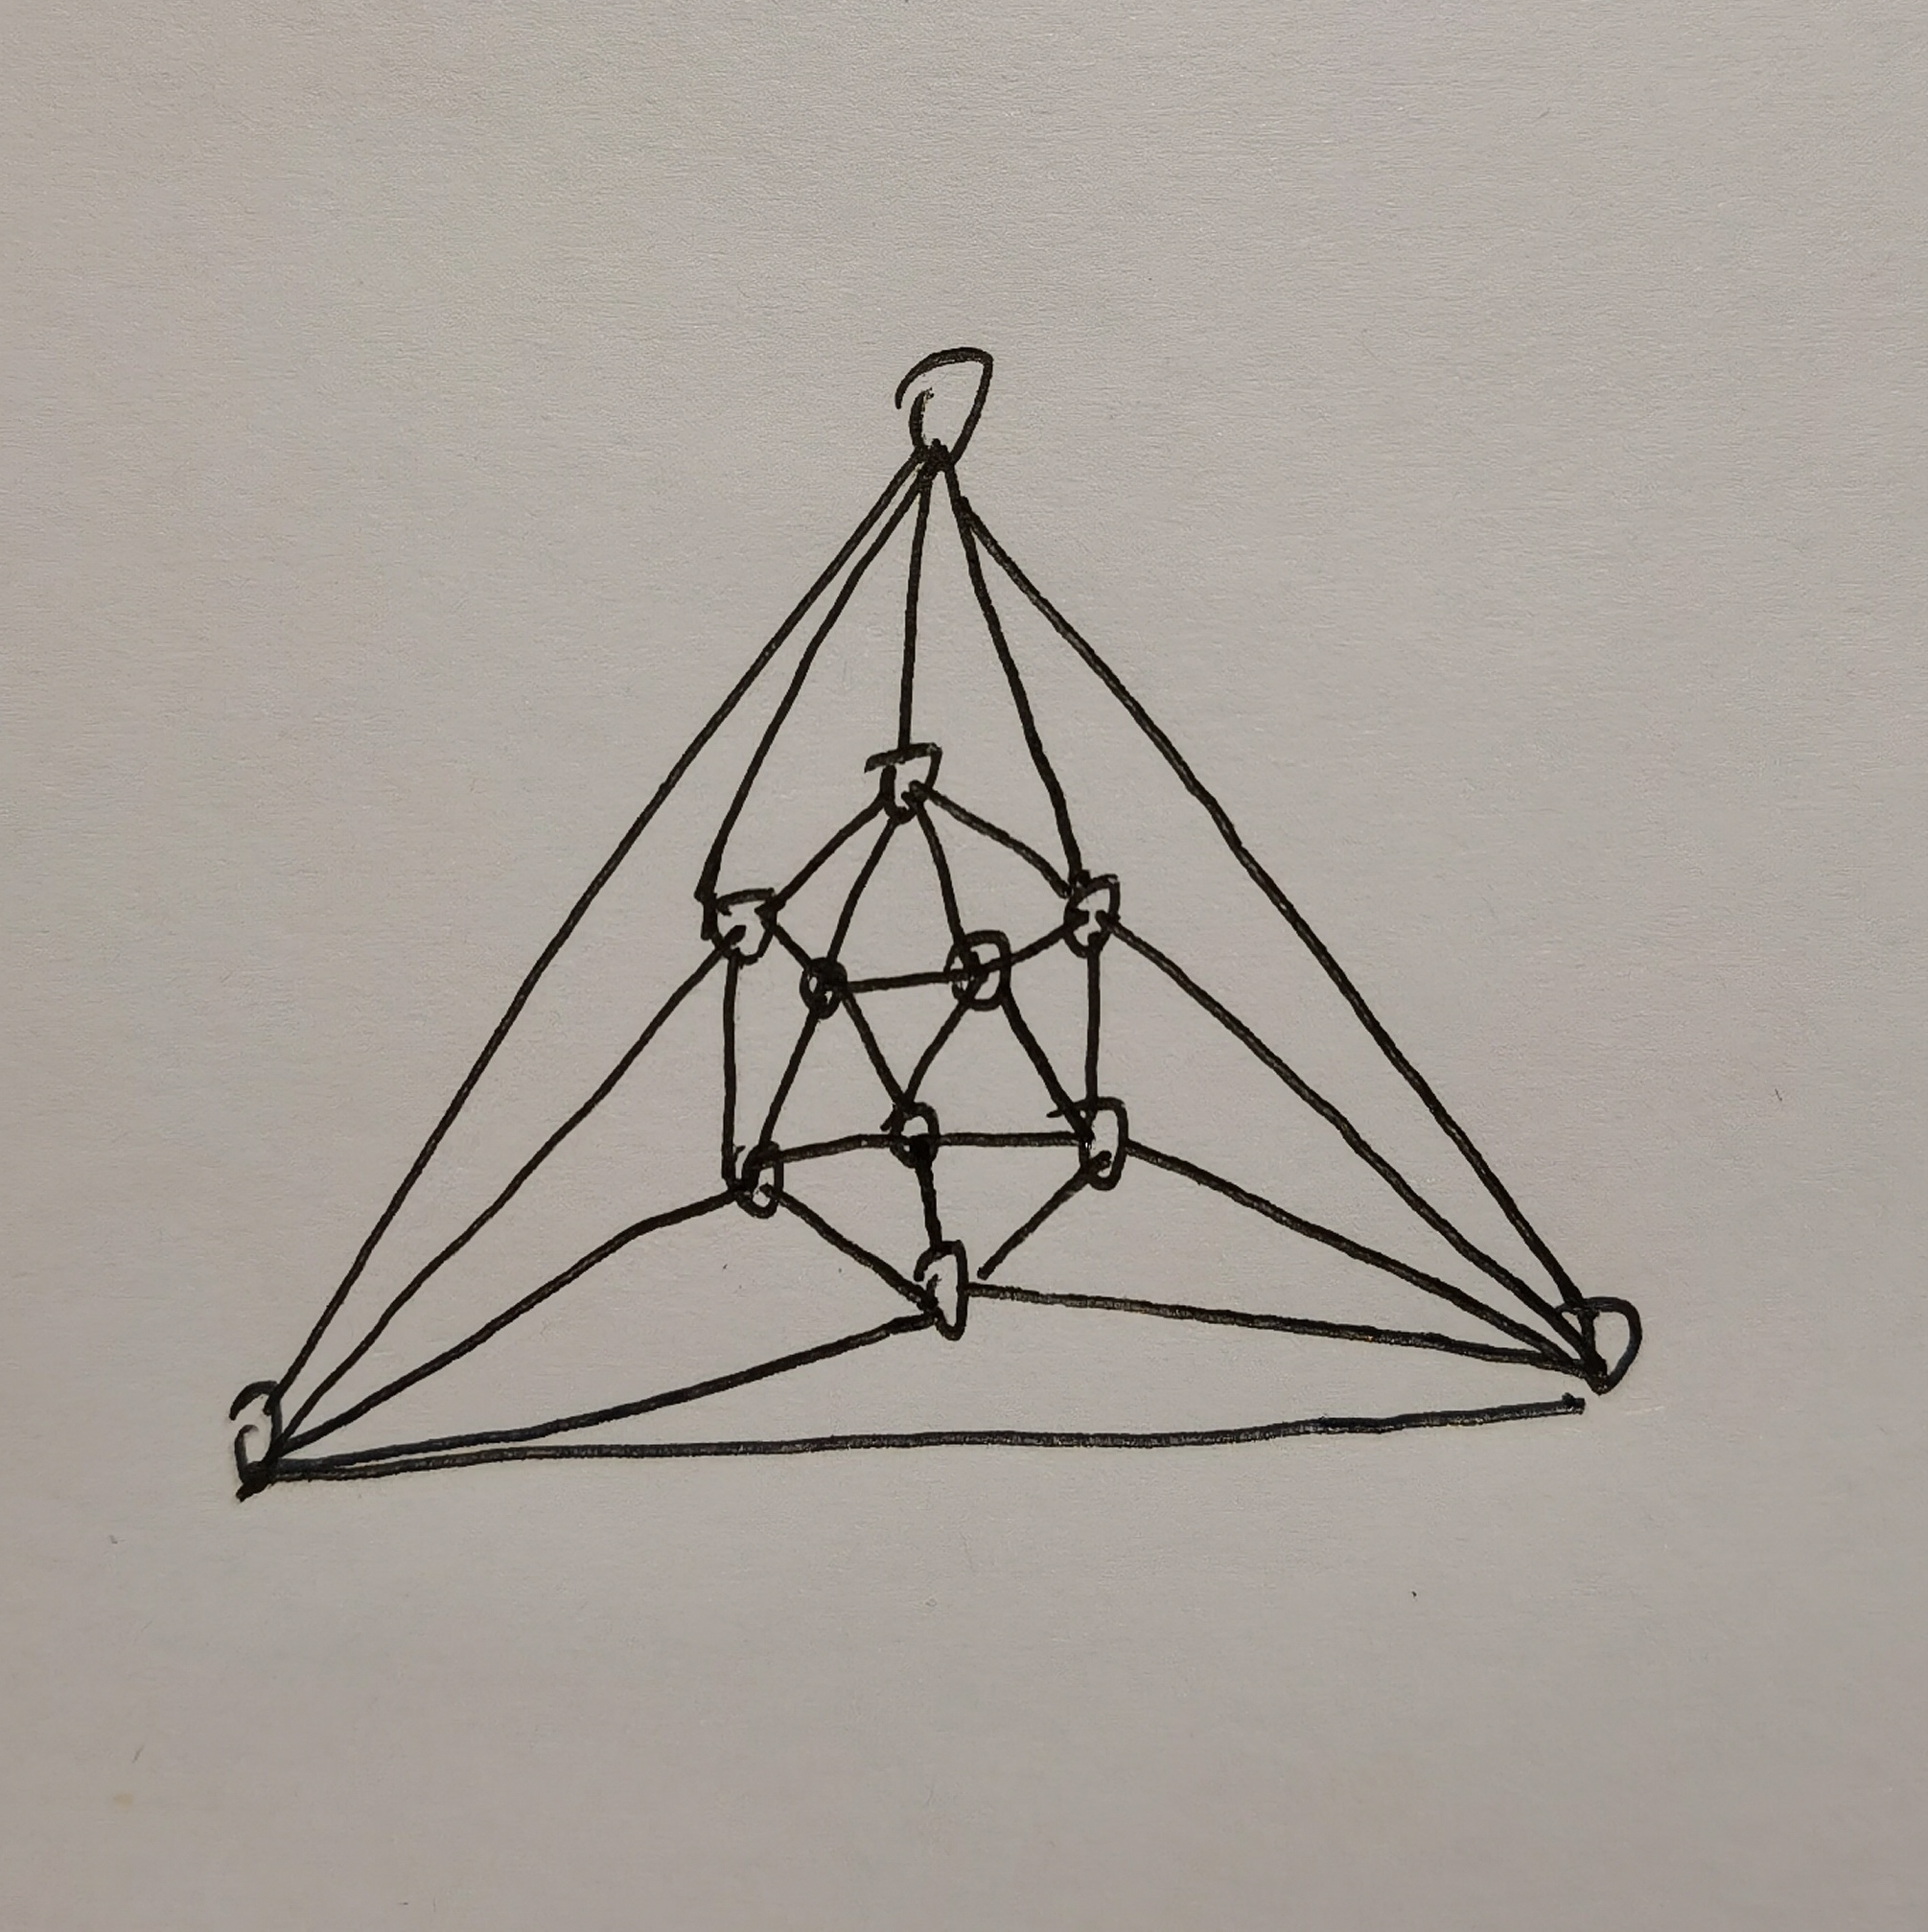
\includegraphics[width = 0.30\linewidth]{figs/b}
  \end{figure}
  \\
  $K_6$\\
  (c)Since $\frac{r\times n}{2} \leq 3n-6$, we can know that there is no r-regular planar graph for $r\geq 6$.
\end{solution}
%%%%%%%%%%%%%%%

%%%%%%%%%%%%%%%
\begin{problem}[CZ 9.7]

\end{problem}

\begin{solution}
  (a)$C_4$\\
  (b)There is no such graph.The graph of order 4 doesn't include $K_{3,3},K_5$ and subgraphs for their segmentation.\\
  (c)
  \begin{figure}[htbp]
    \centering
    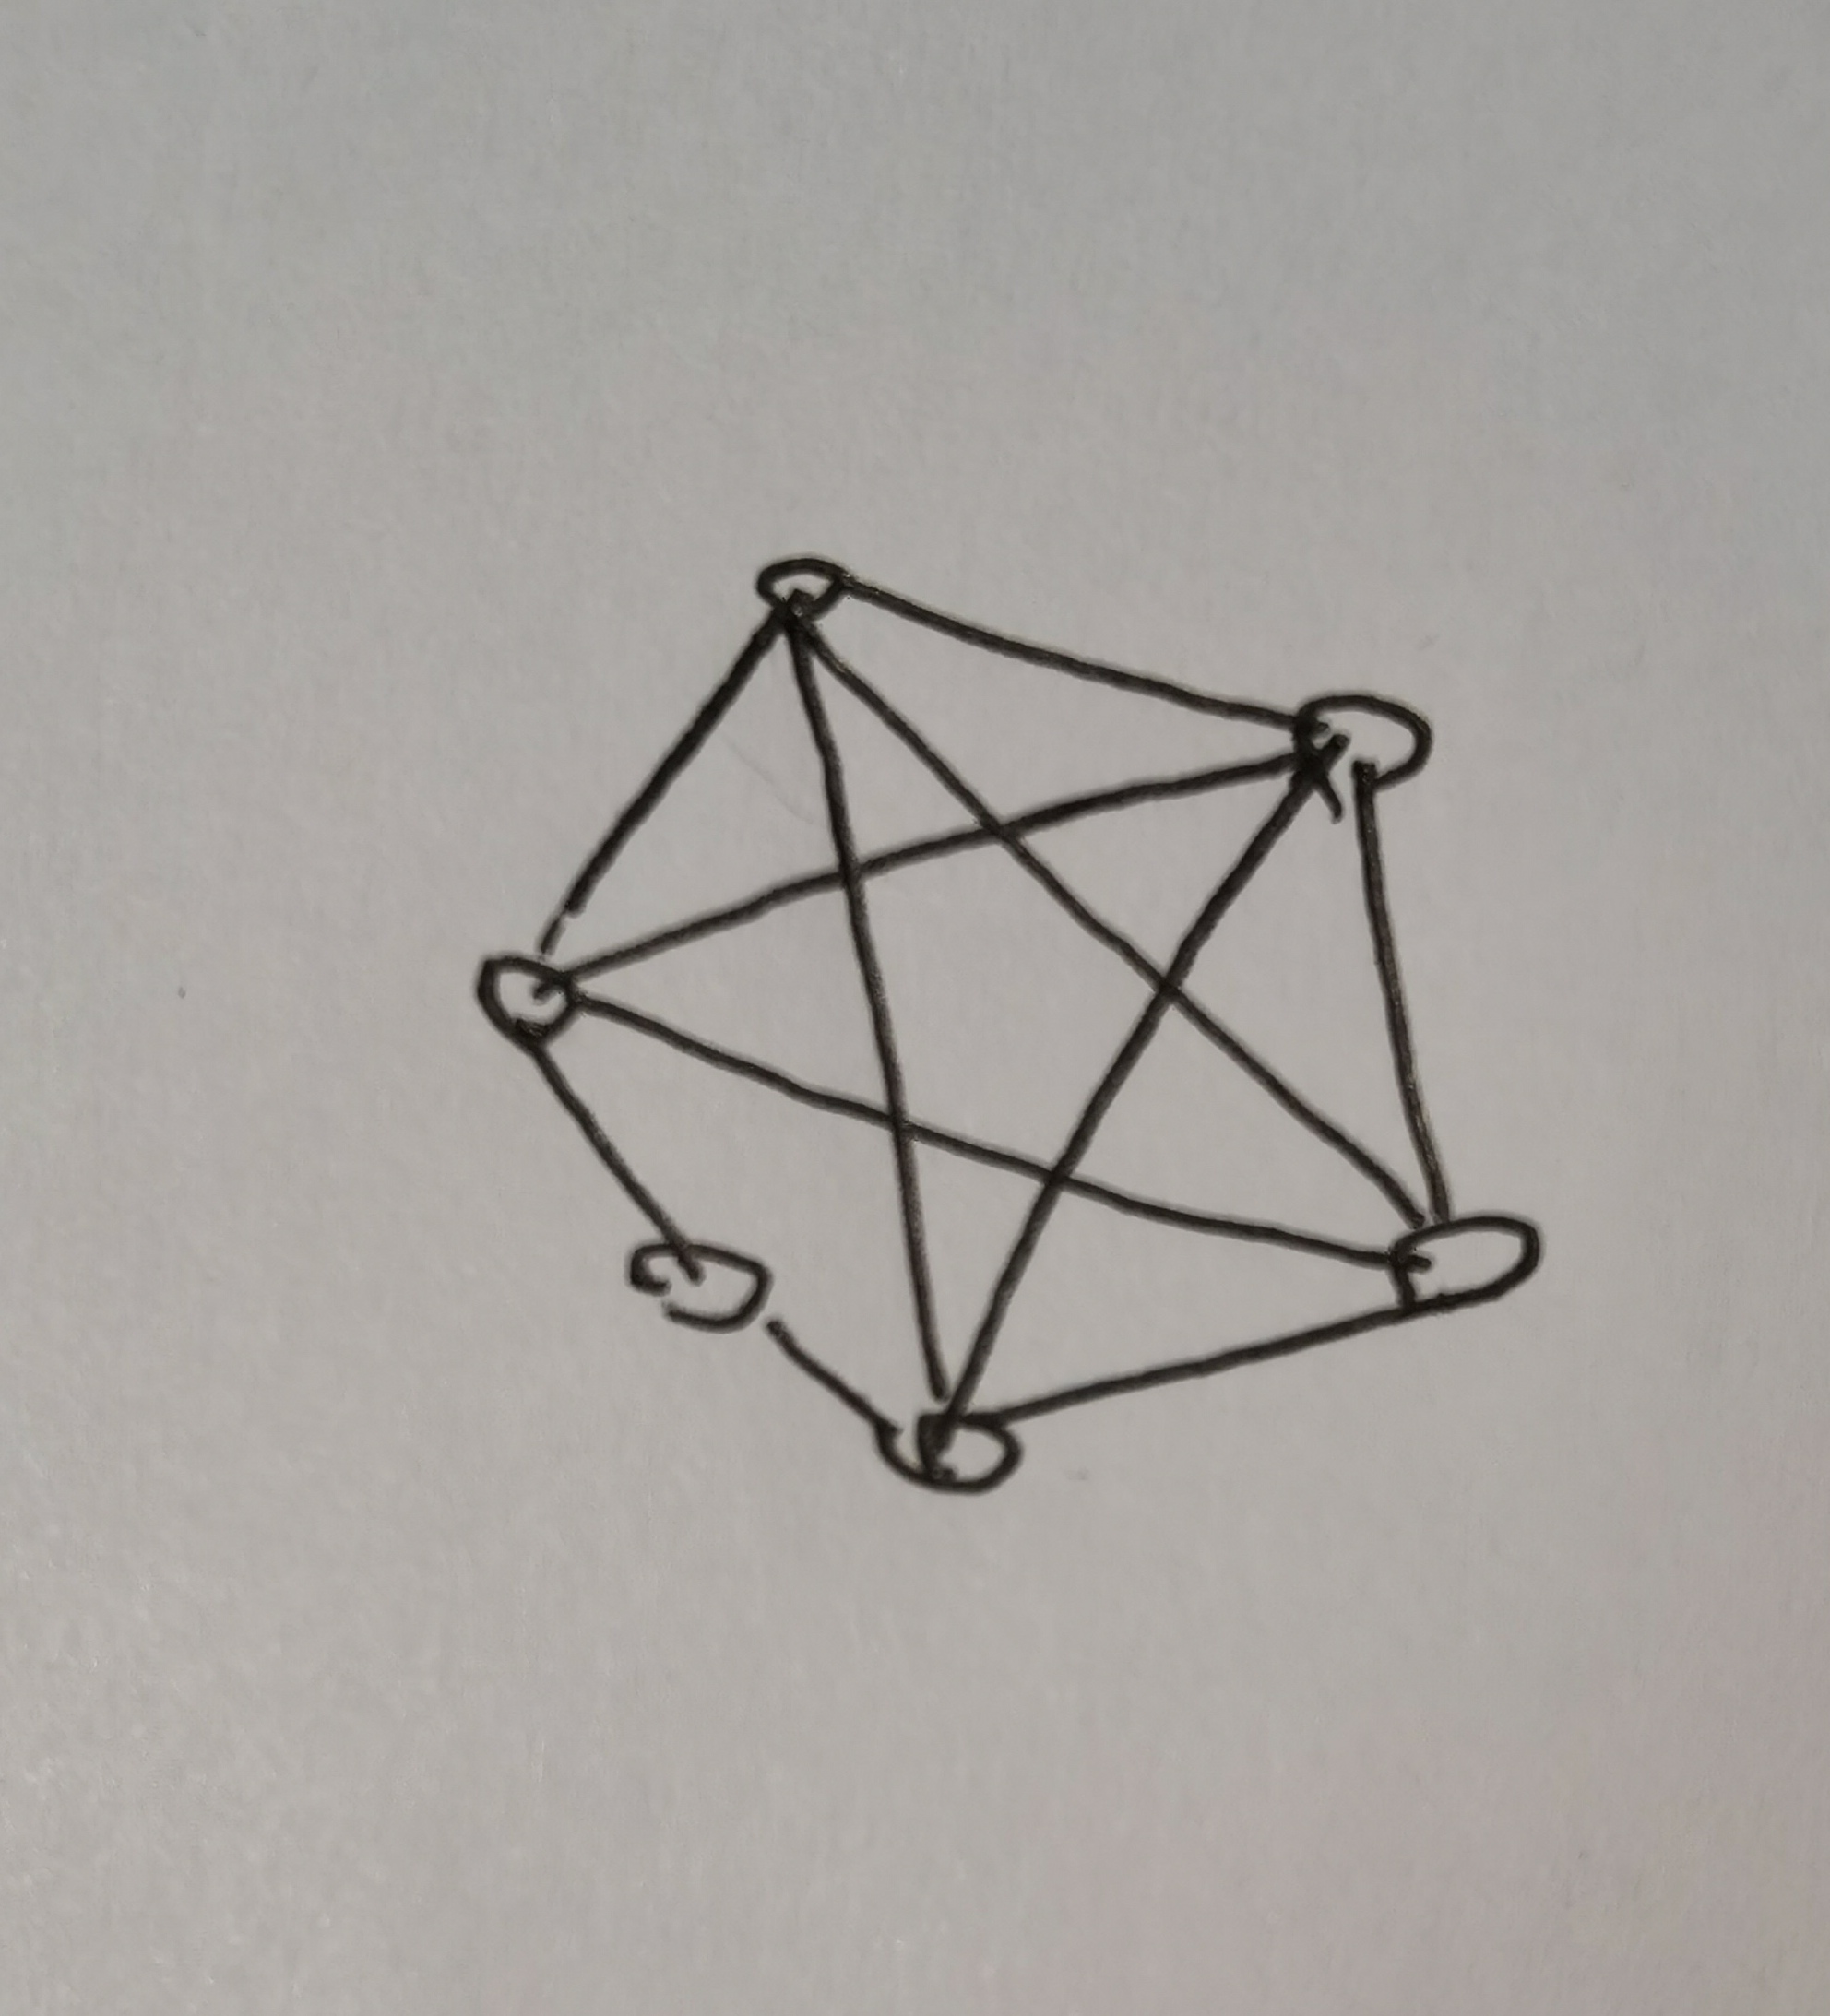
\includegraphics[width = 0.30\linewidth]{figs/c}
  \end{figure}\\
  (d)Since $n=5,m=10$, we can know it is $K_5$. So it can not be a planar graph.\\
  (e)$C_3$\\
  (f)\begin{figure}[htbp]
    \centering
    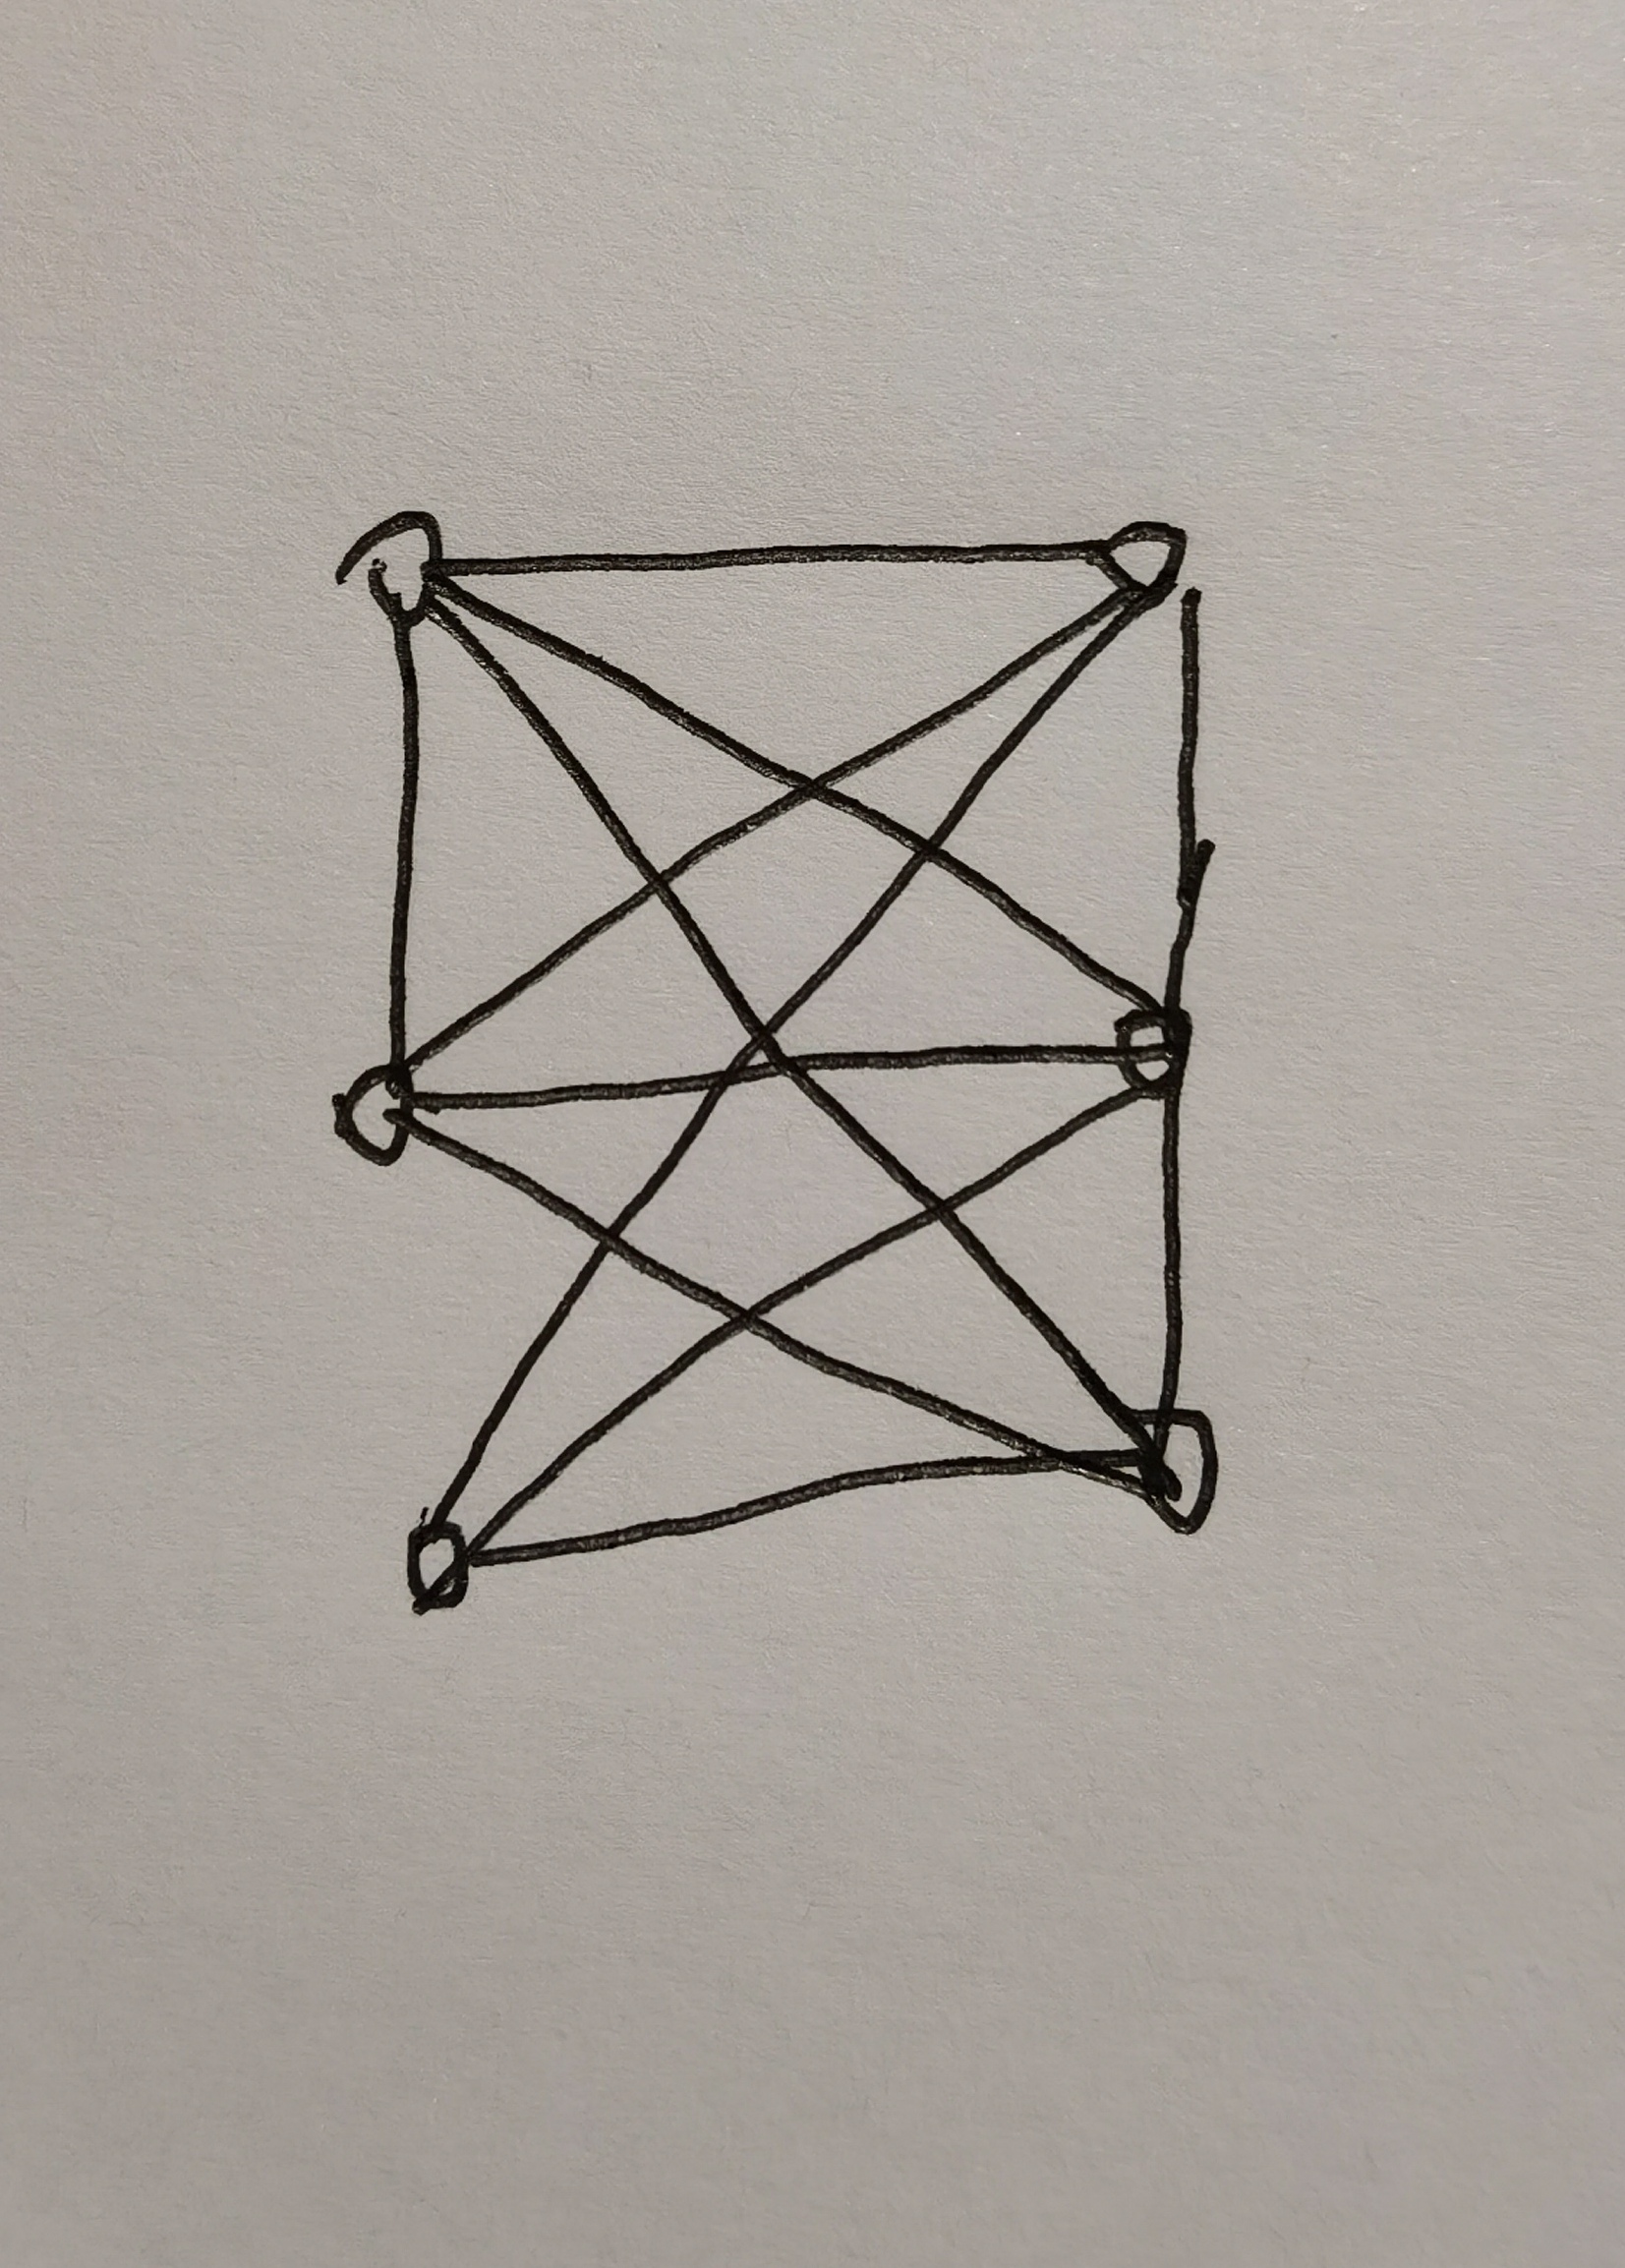
\includegraphics[width = 0.30\linewidth]{figs/d}
  \end{figure}\\
\end{solution}
%%%%%%%%%%%%%%%

%%%%%%%%%%%%%%%
\begin{problem}[CZ 9.8]
\end{problem}

\begin{solution}
  $G=K_4\times K_2$ can not be a planar graph.\\
  The subgraph of $K_4 \times K_2$ contains a breakdown of $K_5$, as shown in the figure.\\
  \begin{figure}[htbp]
    \centering
    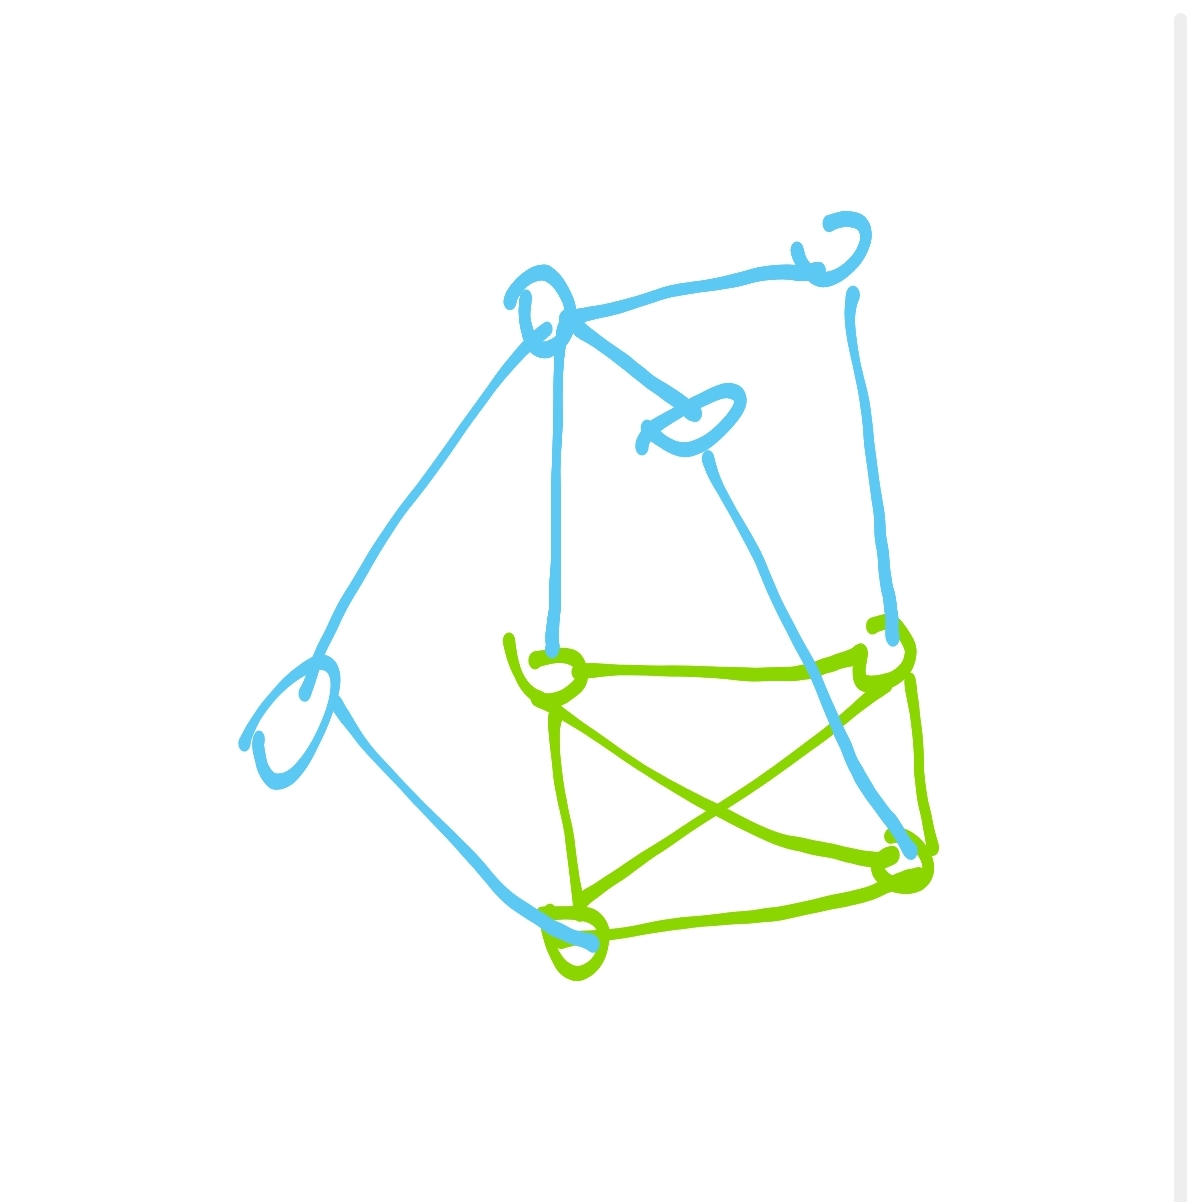
\includegraphics[width = 0.30\linewidth]{figs/e}
  \end{figure}\\
\end{solution}
%%%%%%%%%%%%%%%


%%%%%%%%%%%%%%%
\begin{problem}[CZ 10.2]
\end{problem}

\begin{solution}
  (a)
  If the maximum degree of the Petersen diagram is 3 and contains odd circles, its color number is 3.\\
  (b)
  n-cube is a bipartite with a color number of 2\\
  (c)
  When $n=1$, it is the number of color 2.\\
  $n > 1$ and $n$ is even, the number of colors is 3.\\
  $n > 1$ and $n$ is odd, the color number is 4.
\end{solution}
%%%%%%%%%%%%%%%

%%%%%%%%%%%%%%%
\begin{problem}[CZ 10.3]
\end{problem}

\begin{solution}
  If there is only 1 point, the number of colors is 1. Otherwise, the number of colors is 2.\\
\end{solution}
%%%%%%%%%%%%%%%

%%%%%%%%%%%%%%%
\begin{problem}[CZ 10.4]
\end{problem}

\begin{solution}
  (a)
  No, $K_4$ is a counterexample. \\
  (b)
  No, $C_4$ is a counterexample. \\
  (c)
  No, $K_2$ is a counterexample. \\
  (d)
  No, $K_{3,3}$ is a counterexample.
\end{solution}
%%%%%%%%%%%%%%%

%%%%%%%%%%%%%%%
\begin{problem}[CZ 10.5]
\end{problem}

\begin{solution}
  Suppose it can be divided into three independent sets of $ V_1, V_2, V_3 $. \\
  Generally assumes $ | v_1 | \geq | v_2 | \geq | V_3 | $. \\
  If $ | v_1 | \geq 3 $, the number of edges is $ \leq | k_6 |-| k_ {v_1} | = 12 $ \\
  Otherwise, $ | v_1 | = | v_2 | = | v_3 | = 2 $, then number of edges $ \geq | K_6 | -3 = 12 $
\end{solution}
%%%%%%%%%%%%%%%
%%%%%%%%%%%%%%%%%%%%
\beginot
%%%%%%%%%%%%%%%

%%%%%%%%%%%%%%%
\begin{ot}[请证明Brooks定理]
  \textbf{(Brooks’ Theorem)}For every connected graph G that is not an odd cycle or a
  complete graph, $\chi(G) \le \Delta(G)$
\end{ot}

% \begin{solution}
% \end{solution}
%%%%%%%%%%%%%%%

\begin{ot}[Martin Gardner的愚人节礼物]
  《科学美国人》即《Scientific American》,是美国出版的一种著名科学杂志,在国际上极富声誉。该刊1975年4月号上登载了著
  名数学专栏作家,马丁·加德纳(Martin Gardner)的一篇文章。文章附了一张有着110个区域的地图:
  \fig{width=0.5\linewidth}{figs/Martin-Gardner-fool‘s-day-gift.png}

  加德纳在该图下赫然写道:“四色定理被推翻了!”正文中他还语气肯定地说:该地图不能用少于5种颜色使相邻区域着不同颜色。

  请问:四色定理真的被推翻了么?
\end{ot}

% \begin{solution}
% \end{solution}
%%%%%%%%%%%%%%%




% \vspace{0.50cm}
%%%%%%%%%%%%%%%
% \begin{ot}[]
% 
%   \noindent 参考资料:
%   \begin{itemize}
%     \item 
%   \end{itemize}
% \end{ot}

% \begin{solution}
% \end{solution}
%%%%%%%%%%%%%%%

%%%%%%%%%%%%%%%%%%%%
% 如果没有需要订正的题目,可以把这部分删掉

% \begincorrection
%%%%%%%%%%%%%%%%%%%%

%%%%%%%%%%%%%%%%%%%%
% 如果没有反馈,可以把这部分删掉
\beginfb

% 你可以写
% ~\footnote{优先推荐 \href{problemoverflow.top}{ProblemOverflow}}:
% \begin{itemize}
%   \item 对课程及教师的建议与意见
%   \item 教材中不理解的内容
%   \item 希望深入了解的内容
%   \item $\cdots$
% \end{itemize}
%%%%%%%%%%%%%%%%%%%%
% \bibliography{2-5-solving-recurrence}
% \bibliographystyle{plainnat}
%%%%%%%%%%%%%%%%%%%%
\end{document}